
\begin{frame}[fragile]{Performance Quest}
	\begin{itemize}
		\item Fully compiled to native code
        \item Sample level semantics
        \item Specification language
        \item Automatic parallelization
    \end{itemize}
\end{frame}



\begin{frame}[fragile]{Fully compiled to native code}
Faust code:
\begin{lstlisting}
process = _,_ <: +,-;
\end{lstlisting}

Block-diagram:
\begin{center}
    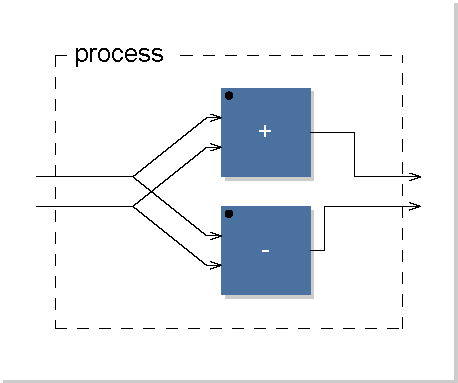
\includegraphics[scale=0.4]{images/expaw}
\end{center}

C++ translation:
\begin{lstlisting}
for (int i = 0; (i < count); i = (i + 1)) {
    float fTemp0 = input0[i];
    float fTemp1 = input1[i];
    output0[i] = fTemp0 + fTemp1;
    output1[i] = fTemp0 - fTemp1;
}
\end{lstlisting}

\end{frame}



\begin{frame}[fragile]{Sample level semantics}
Sawtooth signal by step of $0.01$:
\begin{lstlisting}
decimal = _ <: _, int : -;
process = 0.01 : (+:decimal) ~ _;
\end{lstlisting}

Block-diagram:
\begin{center}
    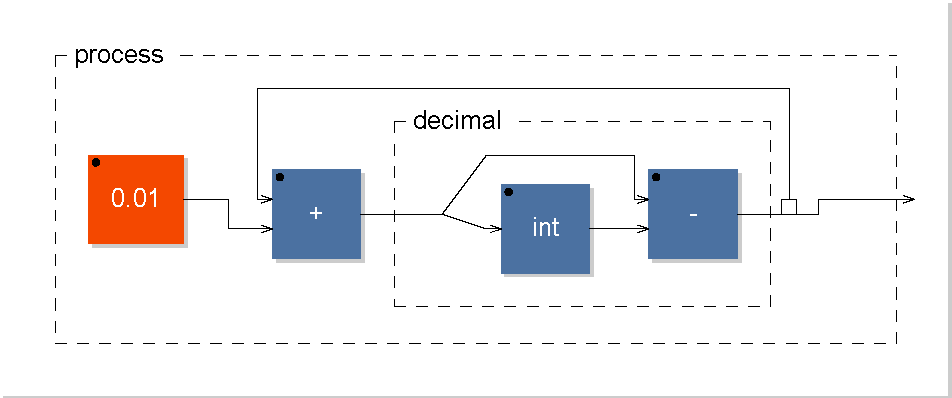
\includegraphics[scale=0.4]{images/sawtooth-diag}
\end{center}

Signal equation:
\begin{eqnarray*}
    y(t<0) & = & 0\\
    y(t\geq 0) & = & decimal(y(t-1) + 0.01)
\end{eqnarray*}

\end{frame}



\begin{frame}[fragile]{Specification Language}{Leave the implementation to the compiler}
User's code:
\begin{lstlisting}
process = _<:(*(0.5):@(2)),(@(1):*(0.5):@(1)):>_;
\end{lstlisting}

Block-diagram:
\begin{center}
    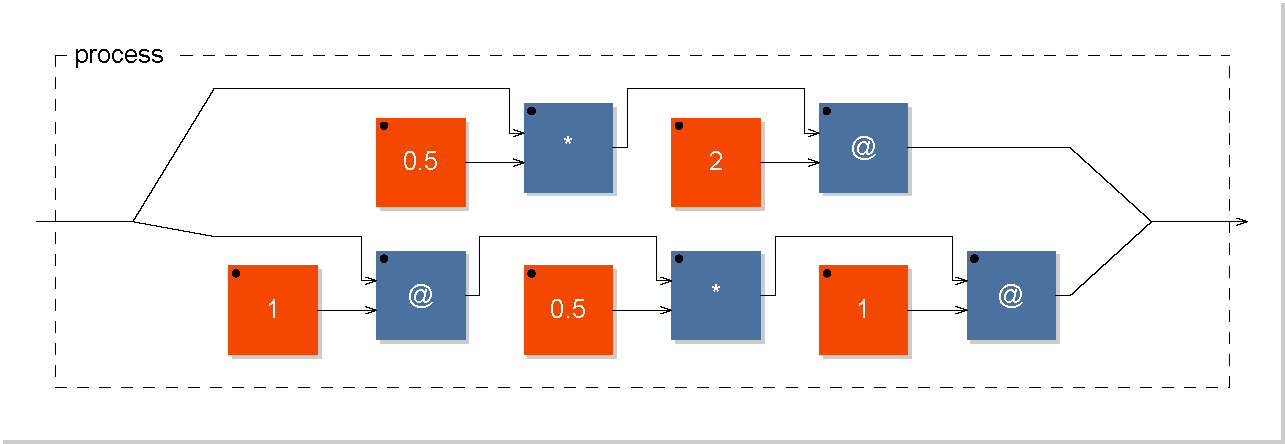
\includegraphics[scale=0.4]{images/equiv1-diag}
\end{center}

Equivalent, more efficient code
\begin{lstlisting}
process = @(2);
\end{lstlisting}

\end{frame}


\begin{frame}[fragile]{Automatic Parallelization}{Code Generators}
    \begin{center}
        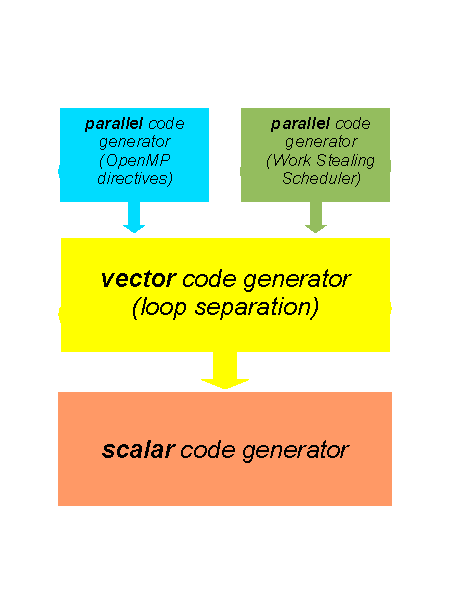
\includegraphics[height=0.75\textheight]{images/compiler-stack1}
    \end{center}
\end{frame}


\begin{frame}[fragile]{Automatic Parallelization}{Performances}
    \begin{center}
        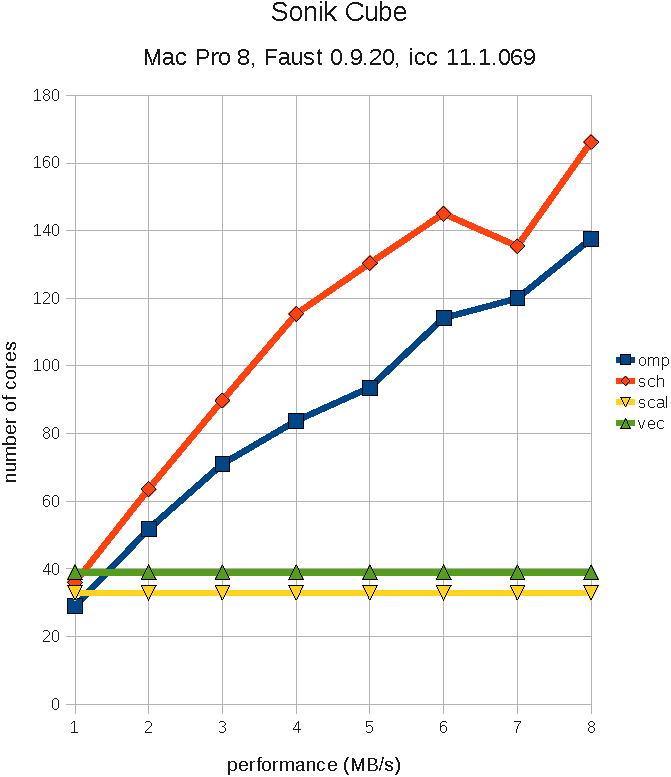
\includegraphics[height=0.75\textheight]{images/ethersonik-bench}
    \end{center}
\end{frame}
